\begin{frame}[t]{Distributed Implemenation}
  \vspace{0.6cm}
  \begin{center}
    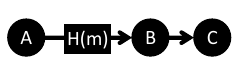
\includegraphics[width=0.50\textwidth]{logic}
  \end{center}
  \begin{itemize}\setlength\itemsep{0.25cm}
    \item A program consists of logical stages (A, B, C)
    \item H(m) controls exchange of data between stages
  \end{itemize}
\end{frame}

\begin{frame}[t]{Data Parallelism}
   \begin{center}
   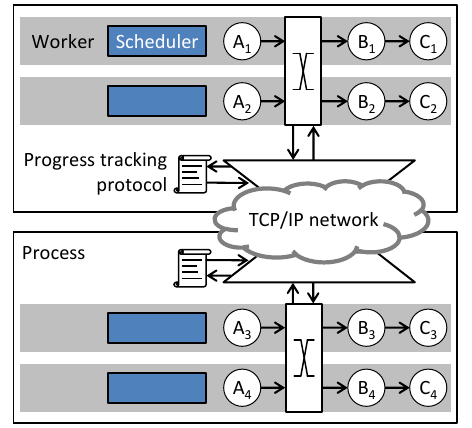
\includegraphics[height=0.4\textwidth]{physical}
   \end{center}
   \begin{itemize}\setlength\itemsep{0.25cm}
     \item Physical graph represents the chosen amount of workers and distributed connected hosts
     \item Programmer can select which way a message should flow in the system
stages
\item Naiad always uses the logical graph as a decision base where data has to flow
    \end{itemize}

\end{frame}

\begin{frame}[t]{Worker}
  \vspace{0.15cm}
  Delivers messages (data) and notifications to vertices

  \begin{itemize}\setlength\itemsep{0.25cm}
    \item Tie-breaker -- Always deliver messages before notifications
    \item Responsible for multiple vertices
    \item Loop data does not pass trough the workers queue
  \end{itemize}

  \pause
  \vspace{0.25cm}
  Synchronization
  \begin{itemize}\setlength\itemsep{0.25cm}
    \item Communicate through shared queue
    \item Queue not necessary if \textsc{SEND/RECV} are under same worker
    \item Re-entrancy due to loops -- enqueue for later, \\
          coalesce incoming messages in \textsc{OnRecv} to reduce memory.
  \end{itemize}

\end{frame}

\begin{frame}[t]{Progress tracking}
\vspace{0.15cm}
\textbf{Problem}: \\
\vspace{0.15cm}
Notification can only be sent if there are no outstanding messages

  \vspace{0.5cm}
  \textbf{Solution}: Own progress tracking protocol
  \begin{itemize}\setlength\itemsep{0.25cm}
     \item Occurence Counters gets updated after a Broadcast to all workers
     \item Local counter never moves ahead of global counter
    \item Allows safe delivery of notifications
   \end{itemize}

\end{frame}

\begin{frame}[t]{Optimizing broadcast updates}
  \vspace{0.15cm}
   \begin{itemize}\setlength\itemsep{0.25cm}
     \item Rely on the logical graph, not the physical.
     \item Buffer before broadcast.
     \item Optimistically first broadcast via UDP to reduce latency.
     \item Wake up threads with either broadcast or unicast with programming primitives.
   \end{itemize}

\end{frame}

 \begin{frame}[t]{Fault tolerance and availability}
  \vspace{0.15cm}
  CHECKPOINT and RESTORE interface
   \begin{itemize}\setlength\itemsep{0.25cm}
     \item Vertex
	 \begin{itemize}\setlength\itemsep{0.25cm}
	 	\item either log data or
        \item full checkpoint when requested
	 \end{itemize}
     \item Progress Tracking Protocoll
     \begin{itemize}\setlength\itemsep{0.25cm}
     	\item full checkpoint
     \end{itemize}
   \end{itemize}

\end{frame}


 \begin{frame}[t]{}
  \vspace{0.15cm}
Tradeoff between Performance and Durability
   \begin{itemize}\setlength\itemsep{0.25cm}
     \item paper favours performance over durablity
     \item Prelies on durable input and output
   \end{itemize}

\end{frame}

 \begin{frame}[t]{Micro Stragglers}
  \vspace{0.15cm}
Naiad is sensitive to latency but tiny interruptions can decrease overall performance  

\begin{tabular}{ l r }
  Iterative Computation & $$<$$ 1 MS \\
  GC, Package loss   & 10th of MS \\
\end{tabular}

Network

\begin{itemize}\setlength\itemsep{0.25cm}
\item Disable Nagle's algorithms
\item Set smaller retry timeout for package loss
\item Use different network protocols in datacenters for computing
\end{itemize}

Garbage Collection

\begin{itemize}\setlength\itemsep{0.25cm}
\item avoid object allocation
\item use buffer pools
\item use value types
\end{itemize}

\end{frame}

 \begin{frame}[t]{Naiad Program}
  \vspace{0.15cm}
   \begin{itemize}\setlength\itemsep{0.25cm}
     \item Provides public API with primitives
     \item Higher Level APIs
     \begin{itemize}\setlength\itemsep{0.25cm}
      \item LINQ
      \item MapReduce
      \item Pregel
     \end{itemize}
     \item Examples do not support coordination
     \begin{itemize}\setlength\itemsep{0.25cm}
     \item to improve performance
     \item concat, distinct, select
     \end{itemize}
     \item Generic API for vertex programming
     \begin{itemize}\setlength\itemsep{0.25cm}
     \item First define the behavior dataflow vertices
     \item Second define the topology
     \end{itemize}
   \end{itemize}

\end{frame}

\begin{frame}[t]{Prototype Program}

\begin{center}
  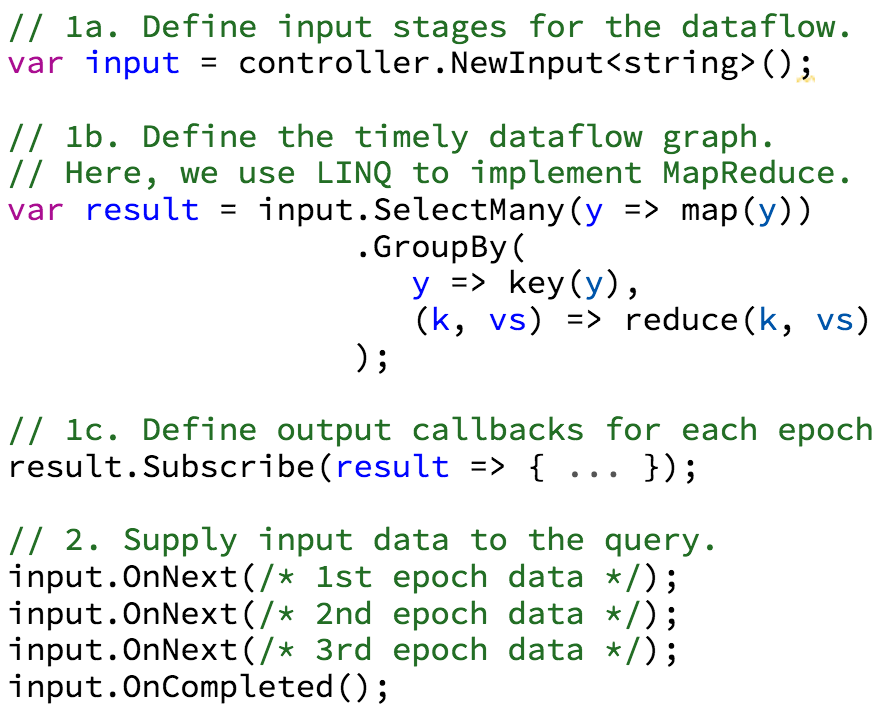
\includegraphics[width=0.9\textwidth]{code}
\end{center}

\end{frame}
